\documentclass[12pt]{article}
\usepackage{geometry} % see geometry.pdf on how to lay out the page. There's lots.
\geometry{a4paper} % or letter or a5paper or ... etc
% \geometry{landscape} % rotated page geometry

% See the ``Article customise'' template for come common customisations
\usepackage{listings}
\usepackage{color}
\usepackage{graphicx}
\usepackage{float}

\definecolor{dkgreen}{rgb}{0,0.6,0}
\definecolor{gray}{rgb}{0.5,0.5,0.5}
\definecolor{mauve}{rgb}{0.58,0,0.82}

\lstset{ % General setup for the package
	language=Java,
	aboveskip=3mm,
	belowskip=3mm,
	showstringspaces=false,
	columns=flexible,
	basicstyle={\small\ttfamily},
	numbers=none,
	numberstyle=\tiny\color{gray},
	keywordstyle=\color{blue},
	commentstyle=\color{dkgreen},
	stringstyle=\color{mauve},
	breaklines=true,
	breakatwhitespace=true,
	tabsize=3
}

\title{Advanced Programming Concepts - Coursework}
\author{Vishnu Sreekumar}
\date{} % delete this line to display the current date

%%% BEGIN DOCUMENT
\begin{document}

\maketitle
\tableofcontents
\newpage

\section{Description}
The application lets the user input the details of the cardboard box order(s) and generate an invoice. If the order cannot be supplied by the company, order is rejected with an error message.

\subsection{Assumptions}
If the user supplies multiple orders and one of the order is not valid or has invalid inputs, the order is not added to the list of orders. If the user decides to proceed, an invoice for the remaining orders (if any) is generated.

\subsection{Limitations}
\begin{enumerate}
	\item[--] Invoice is generated in plain text and there is no built-in print or download options. 
	\item [--] Generated invoices are not saved in application and once the user decide to place a new order, the current order details are reset.
	\item[--] All error and info messages are pop-ups.
\end{enumerate}
\newpage
\section{UML Diagrams}
\subsection{Class Hierarchy Diagram}
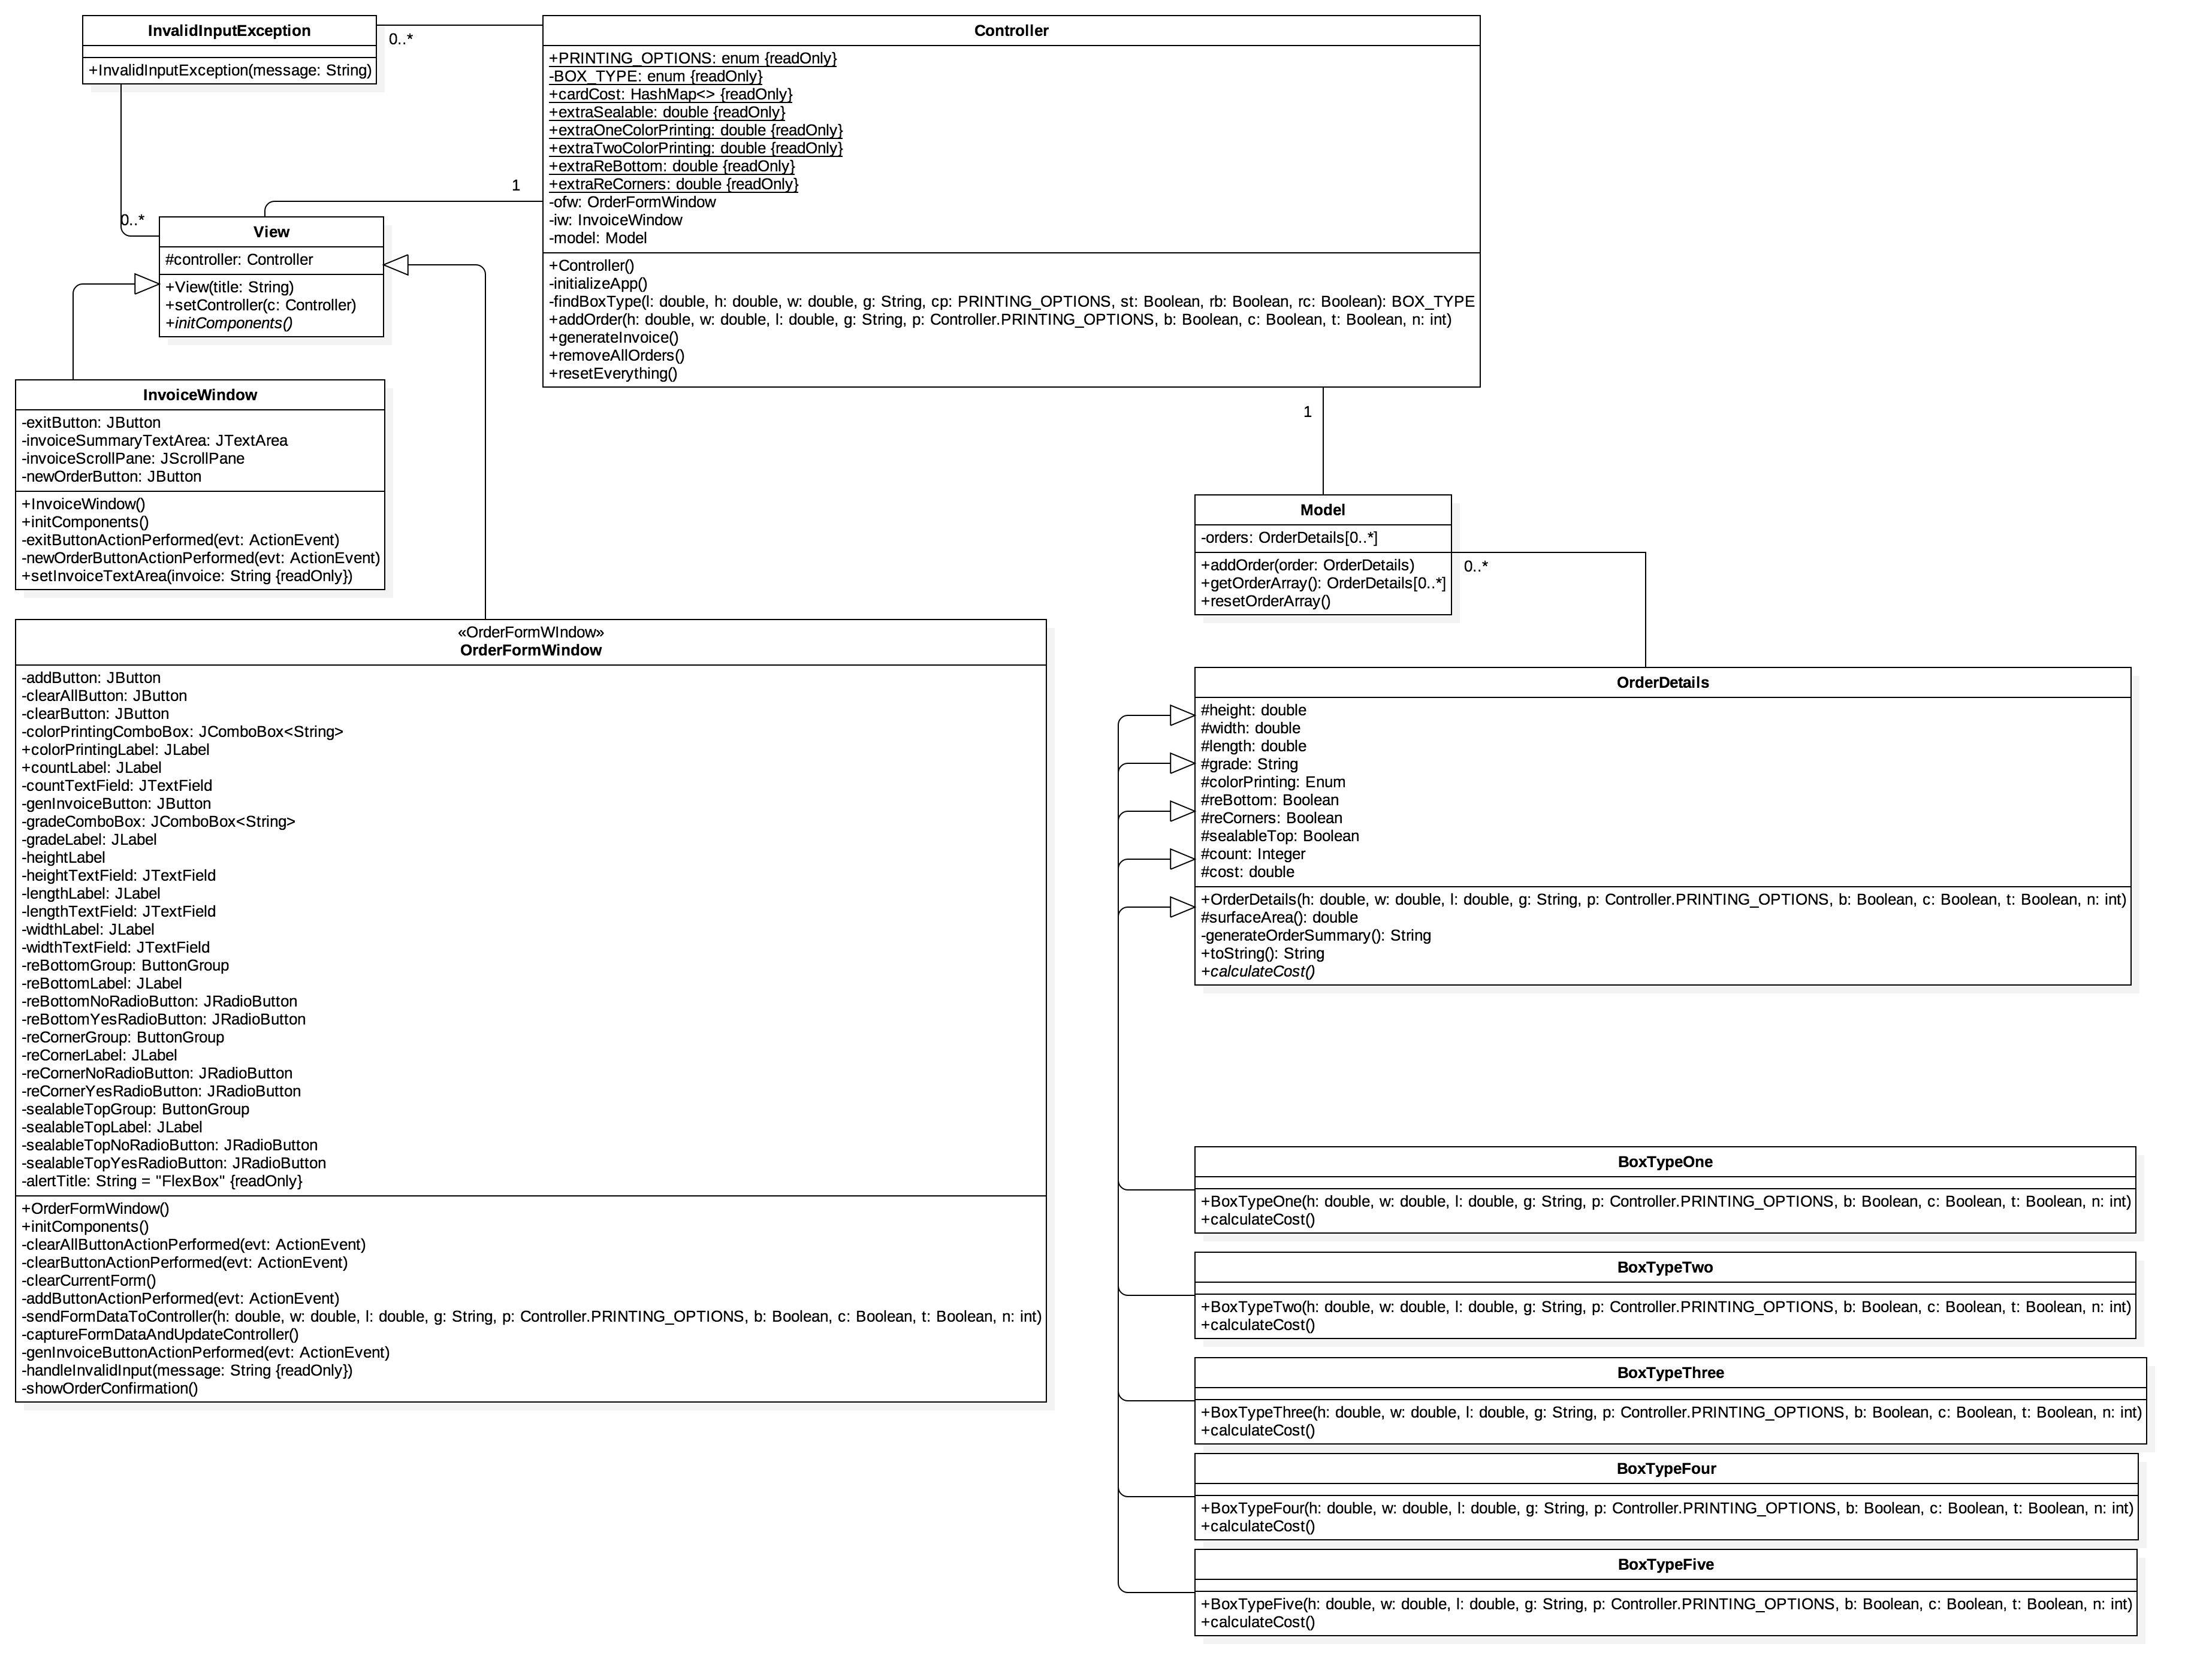
\includegraphics[scale=0.13]{./diagrams/ClassHierarchyDiagram.jpg}
\subsection{Instance Diagram}
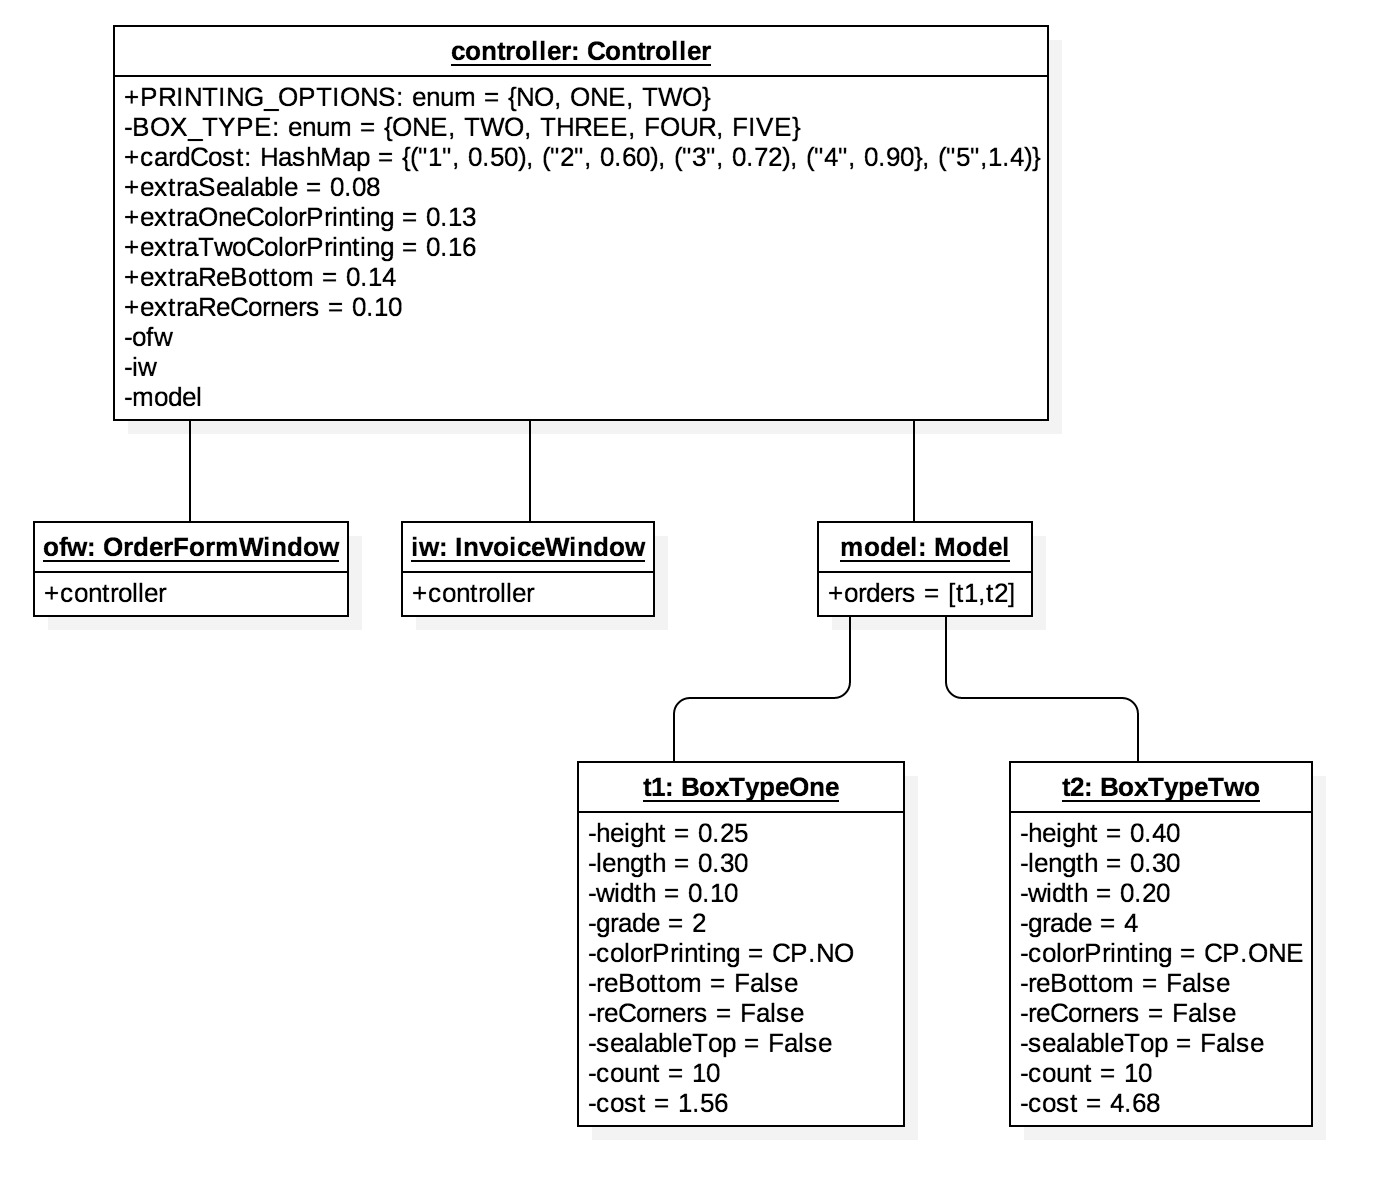
\includegraphics[scale=.3]{./diagrams/InstanceDiagram.jpg}
\subsection{Use Case Diagram}
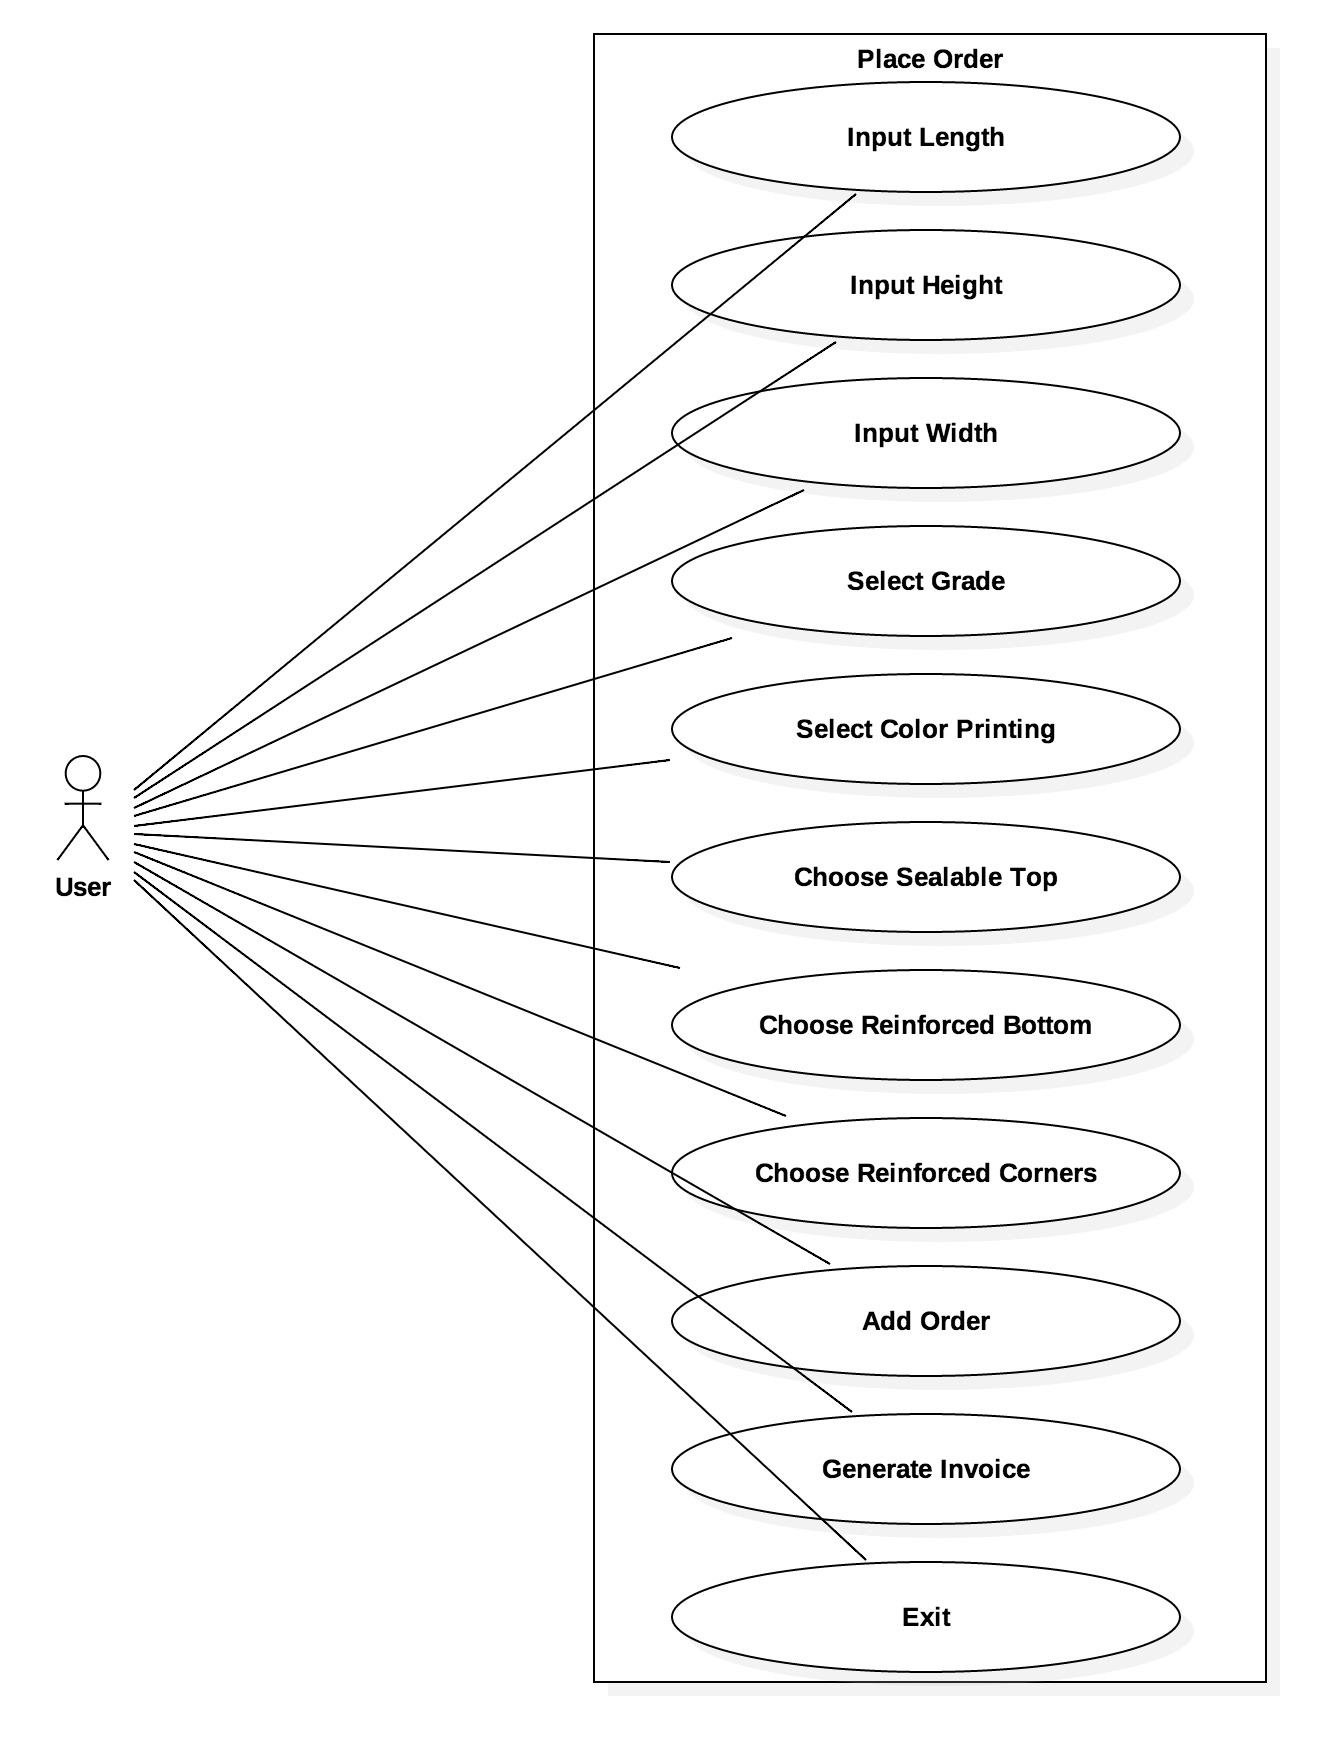
\includegraphics[scale=.30]{./diagrams/UseCaseDiagram.jpg}
\subsection{Sequence Diagram}
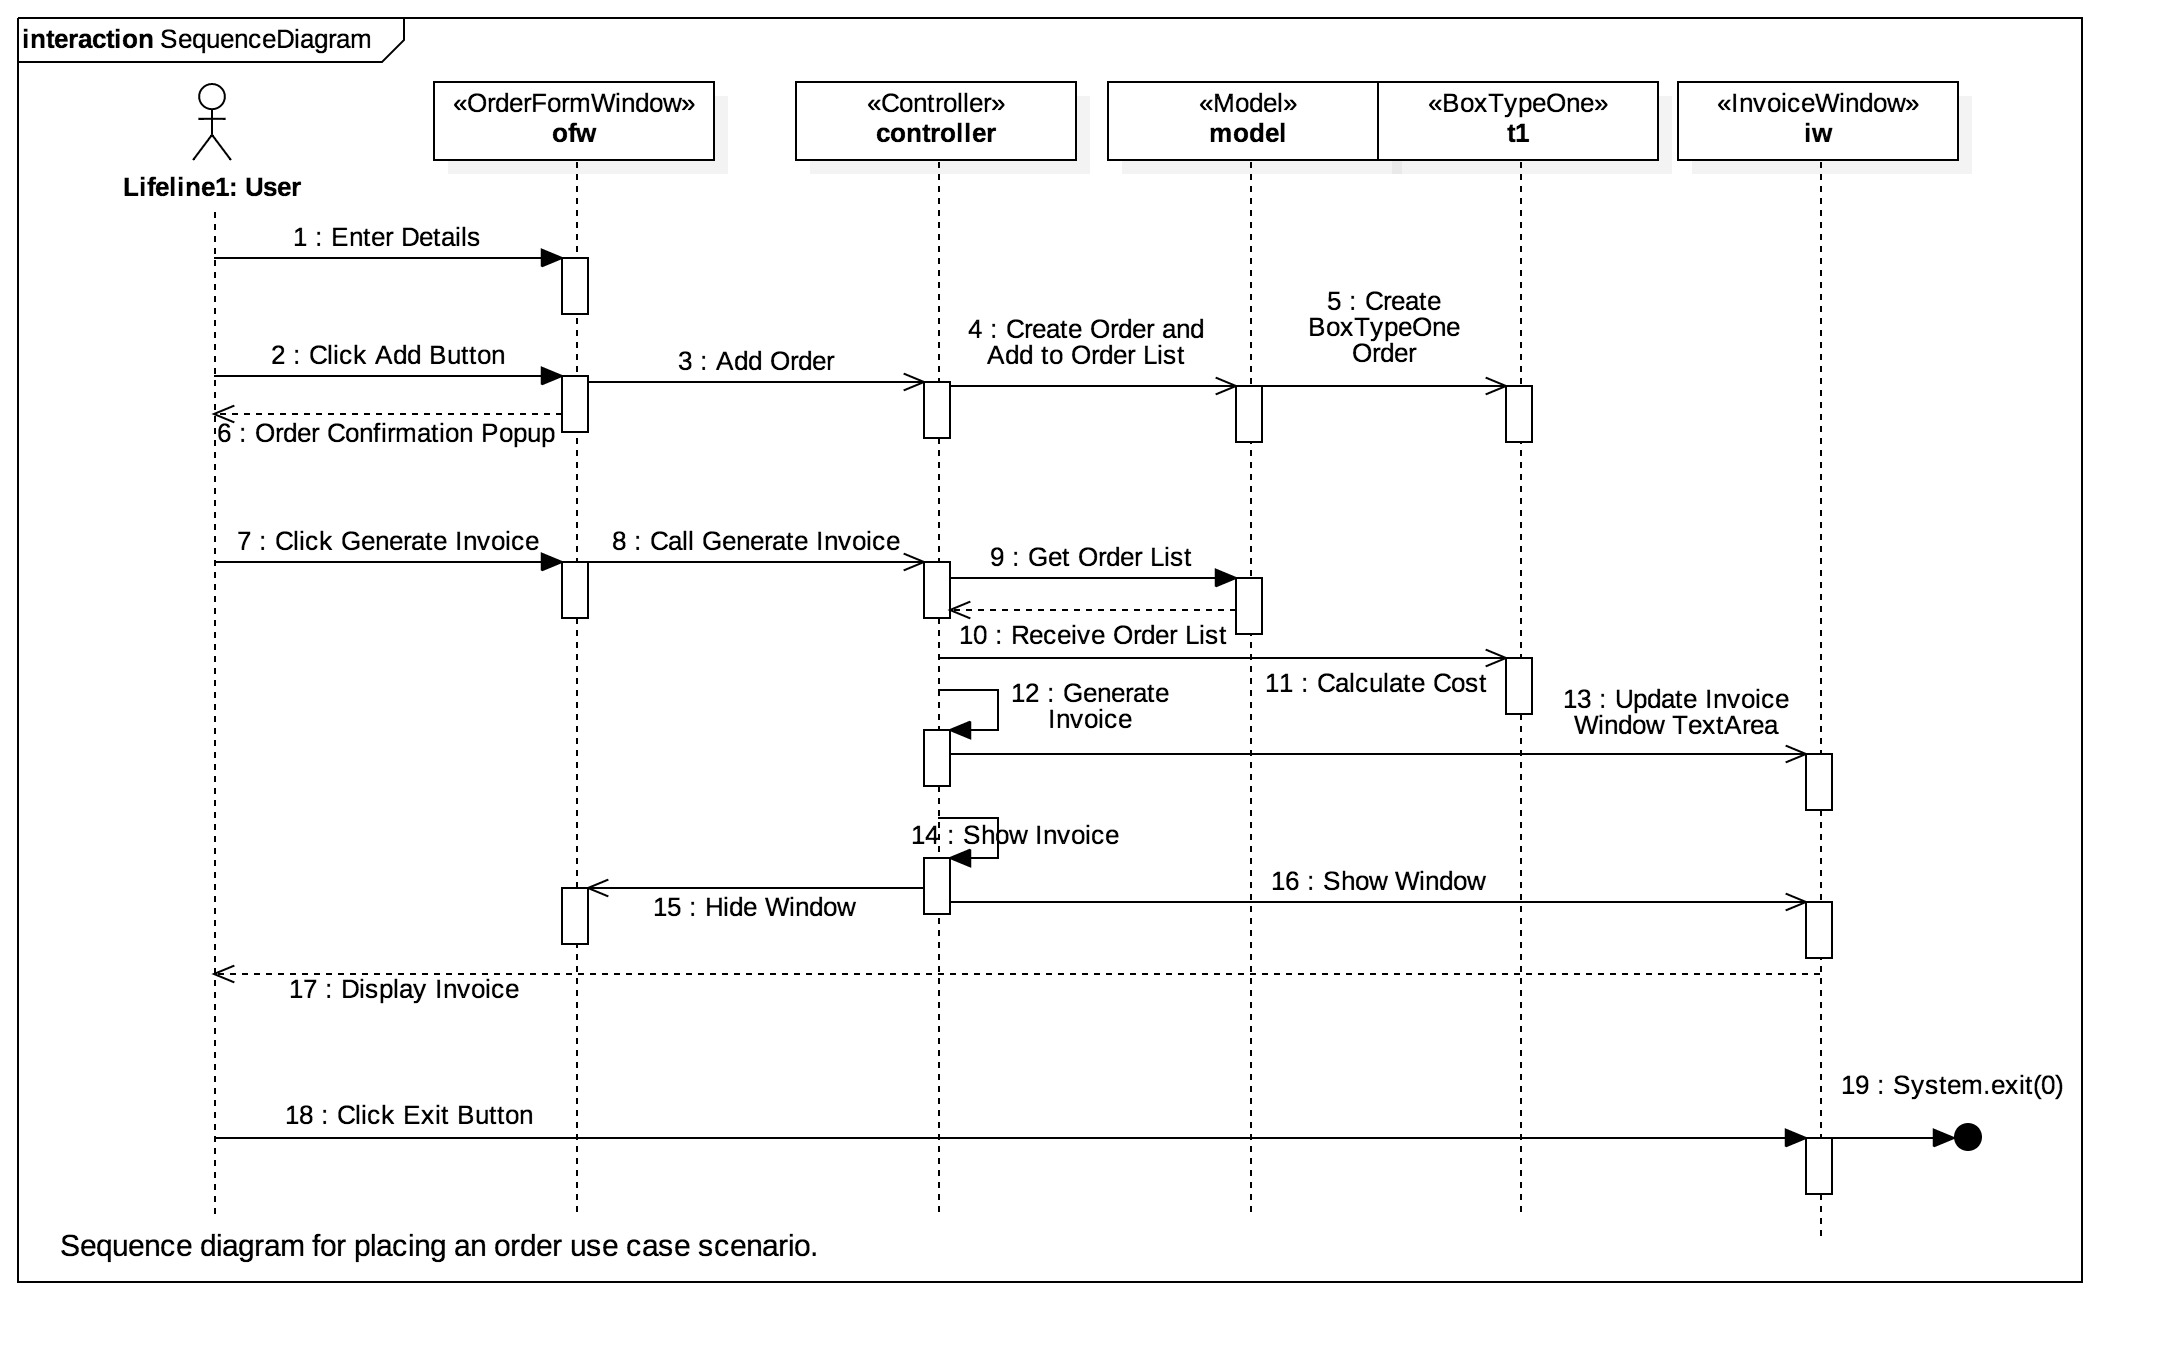
\includegraphics[scale=.20]{./diagrams/SequenceDiagram.jpg}
\newpage
\section{Test Schedule}
\subsection{Test 1}
\subsubsection{Test Case}
Invalid input(s)
\subsubsection{Input}
Length: a\\
Height: .25\\
Width: .30\\
Number of Boxes: 10\\
\subsubsection{Expected Output}
A popup showing error message "Invalid input: Please check the values"
\subsubsection{Screenshots}
\begin{figure}[H]
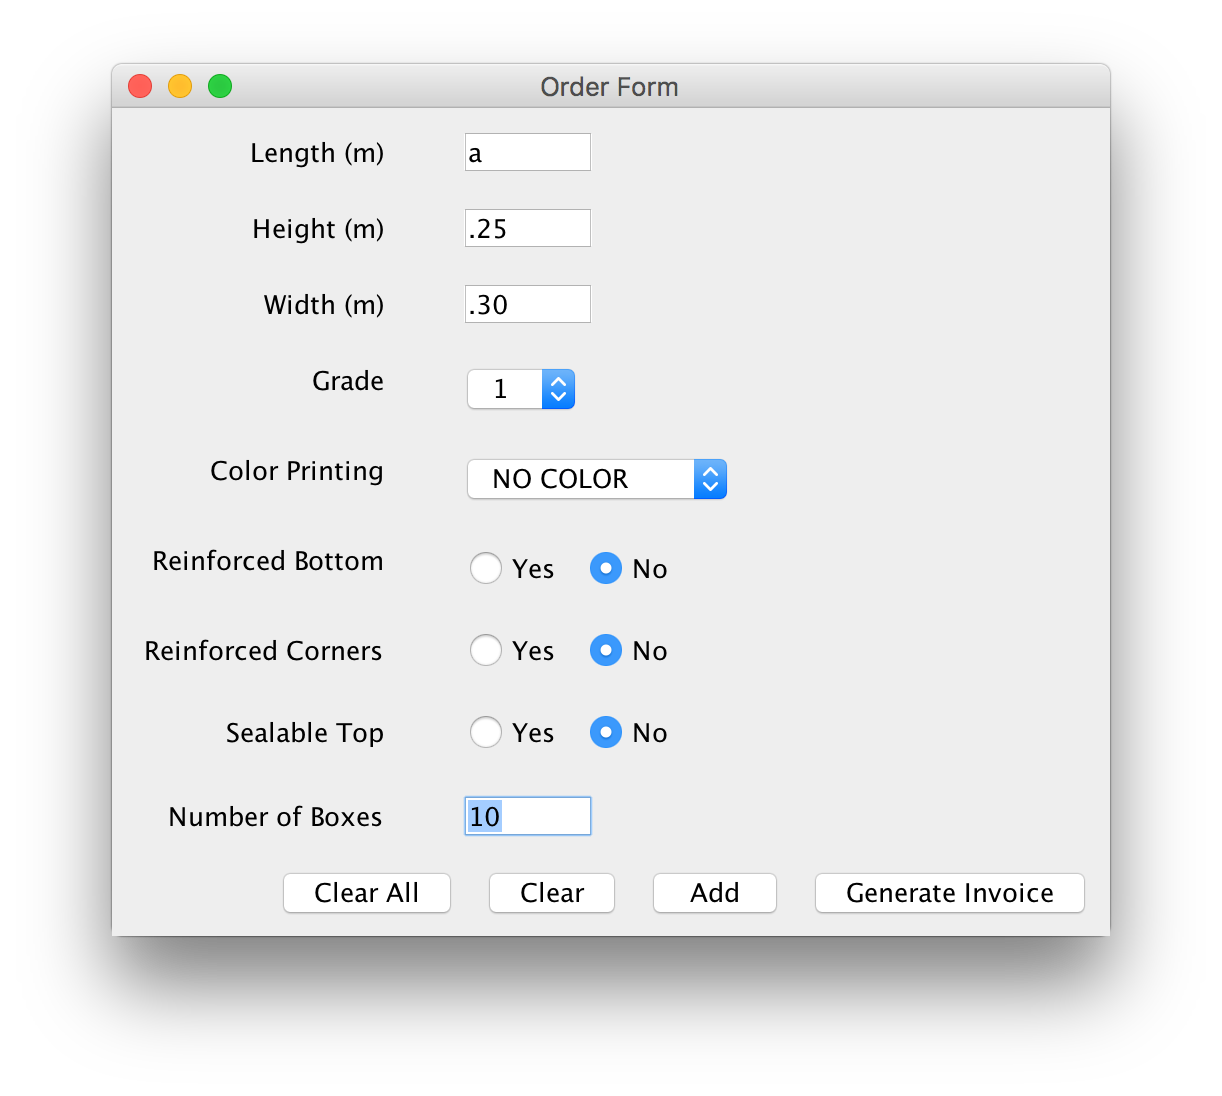
\includegraphics[width=\linewidth]{./screenshots/test_case_1_input.png}
\caption{Test Case 1 Input}
\label{test_case_1_input}
\end{figure}
\begin{figure}[H]
	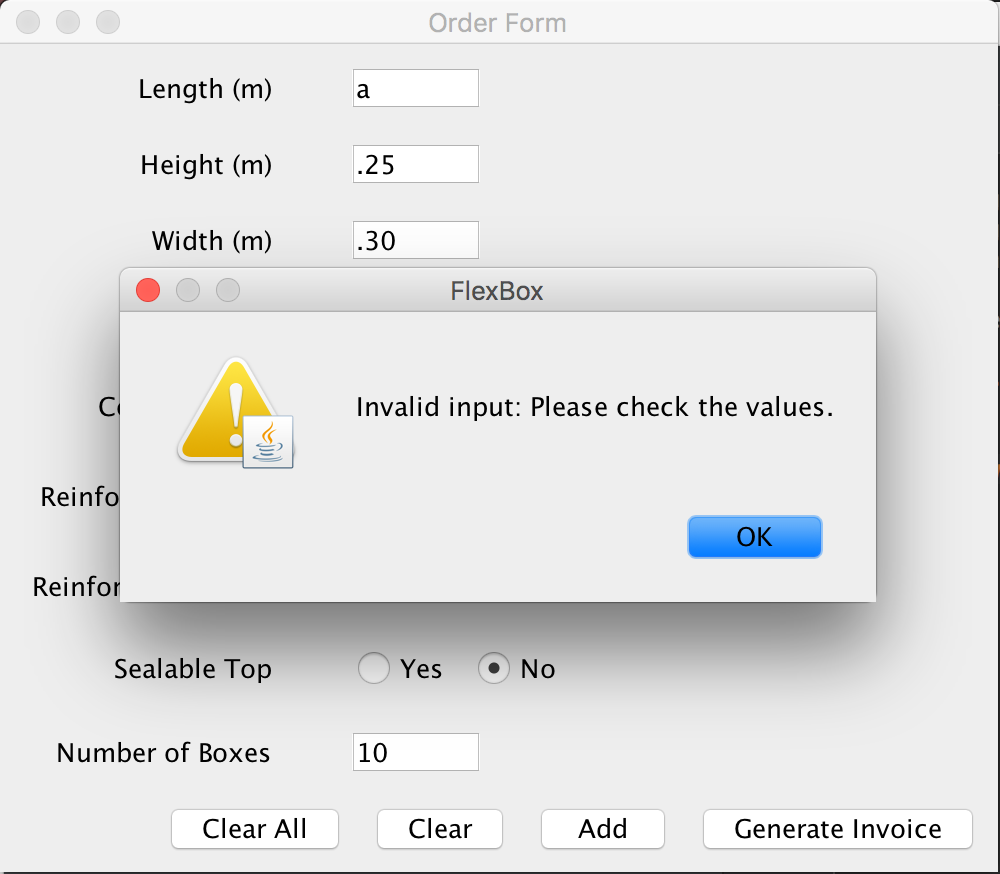
\includegraphics[width=\linewidth]{./screenshots/test_case_1_output.png}
	\caption{Test Case 1 Output}
	\label{test_case_1_output}
\end{figure}
\newpage
\subsection{Test 2}
\subsubsection{Test Case}
Incorrect input
\subsubsection{Input}
Length: 0.20\\
Height: 0.30\\
Widht: 0.25\\
Number of Boxes: 0\\
\subsubsection{Expected Output}
A popup showing error message "Invalid input: Box dimensions and count must be greater than 0"
\subsubsection{Screenshots}
\begin{figure}[H]
	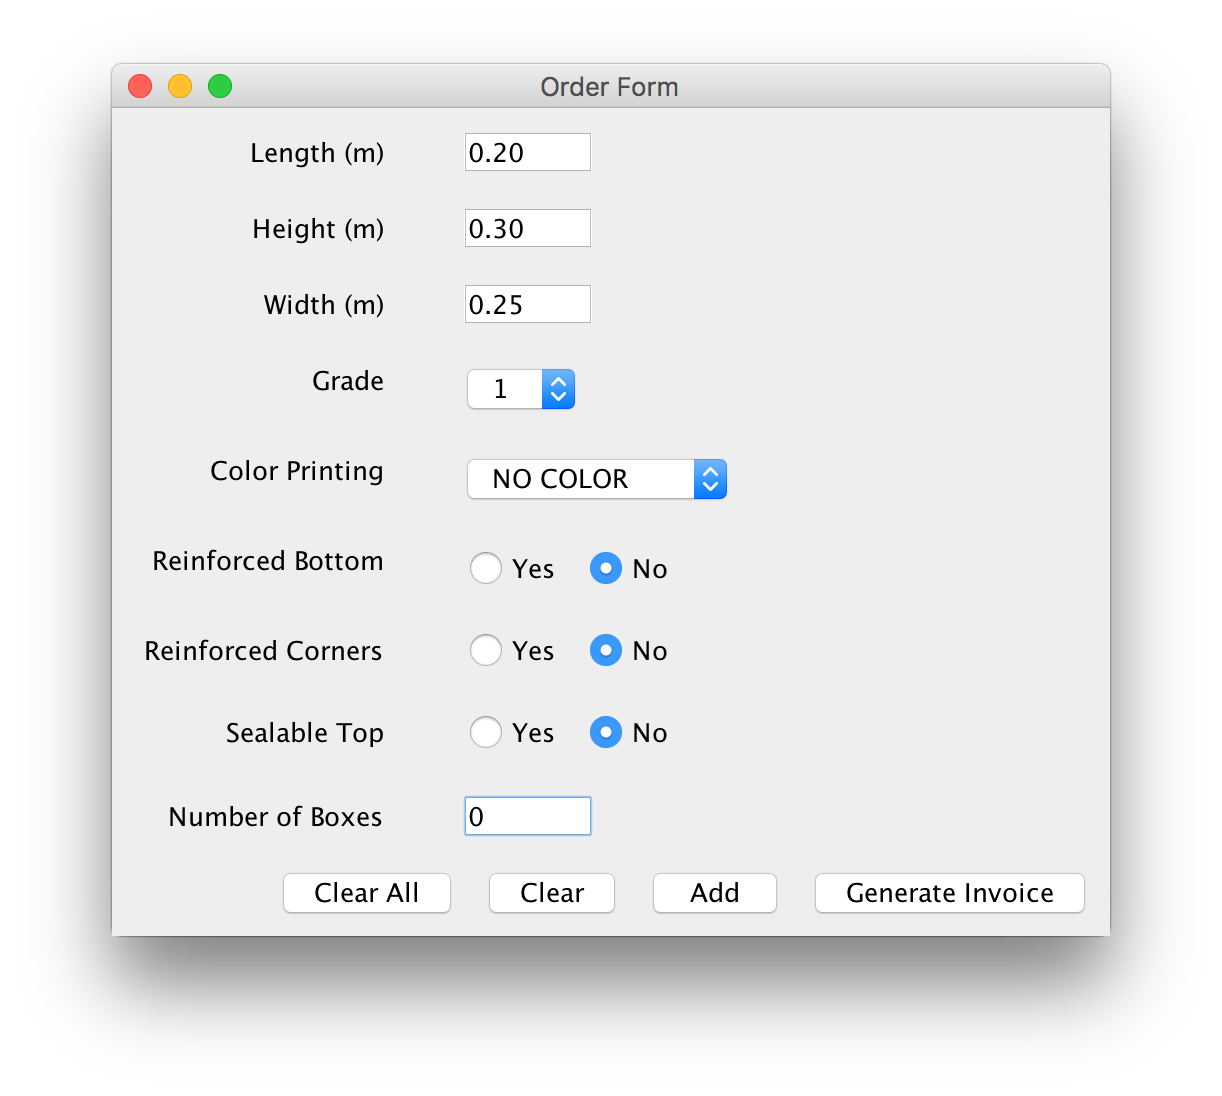
\includegraphics[width=\linewidth]{./screenshots/test_case_2_input.png}
	\caption{Test Case 2 Input}
	\label{test_case_2_input}
\end{figure}
\begin{figure}[H]
	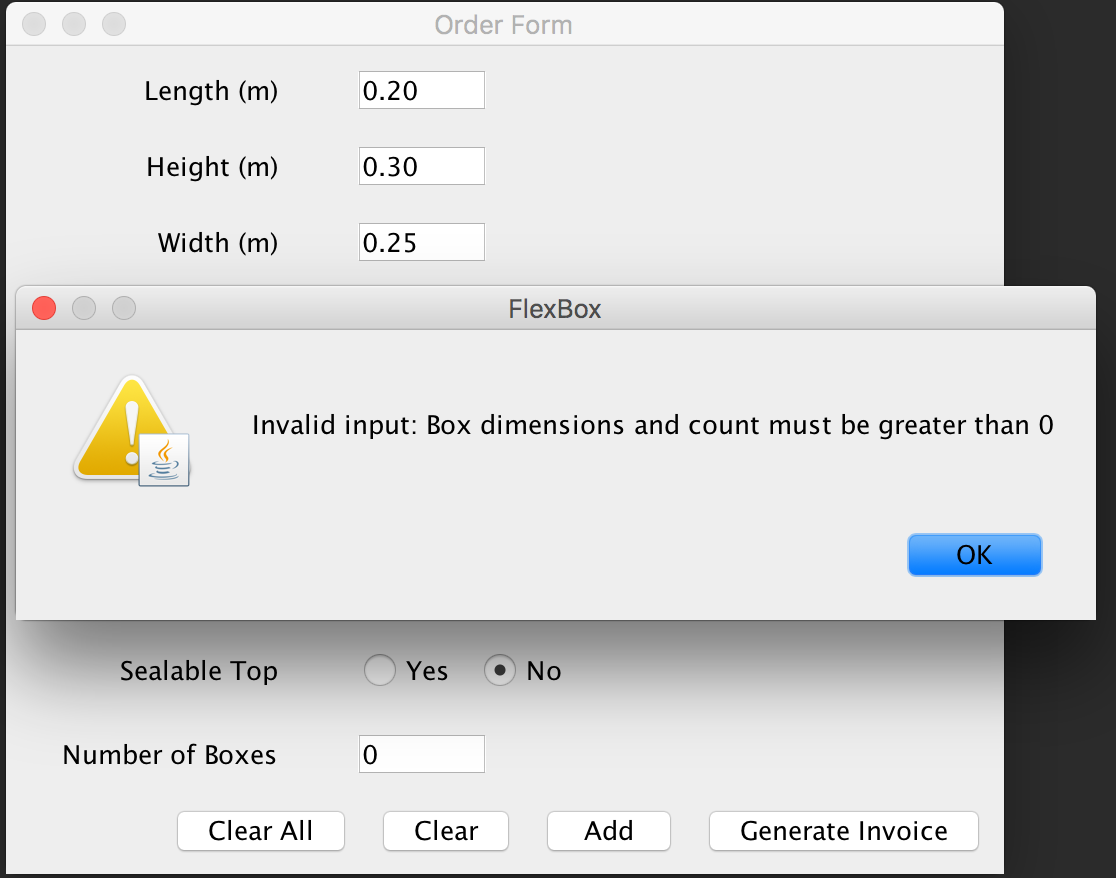
\includegraphics[width=\linewidth]{./screenshots/test_case_2_output.png}
	\caption{Test Case 2 Output}
	\label{test_case_2_output}
\end{figure}
\newpage
\subsection{Test 3}
\subsubsection{Test Case}
Non-suppliable order
\subsubsection{Input}
Length: .10\\
Height: .20\\
Width: .40\\
Grade: 4\\
Reinforced Bottom: Yes\\
Number of Boxes: 10\\
\subsubsection{Expected Output}
A popup showing error message "Sorry, we are not able to supply this order"
\subsubsection{Screenshots}
\begin{figure}[H]
	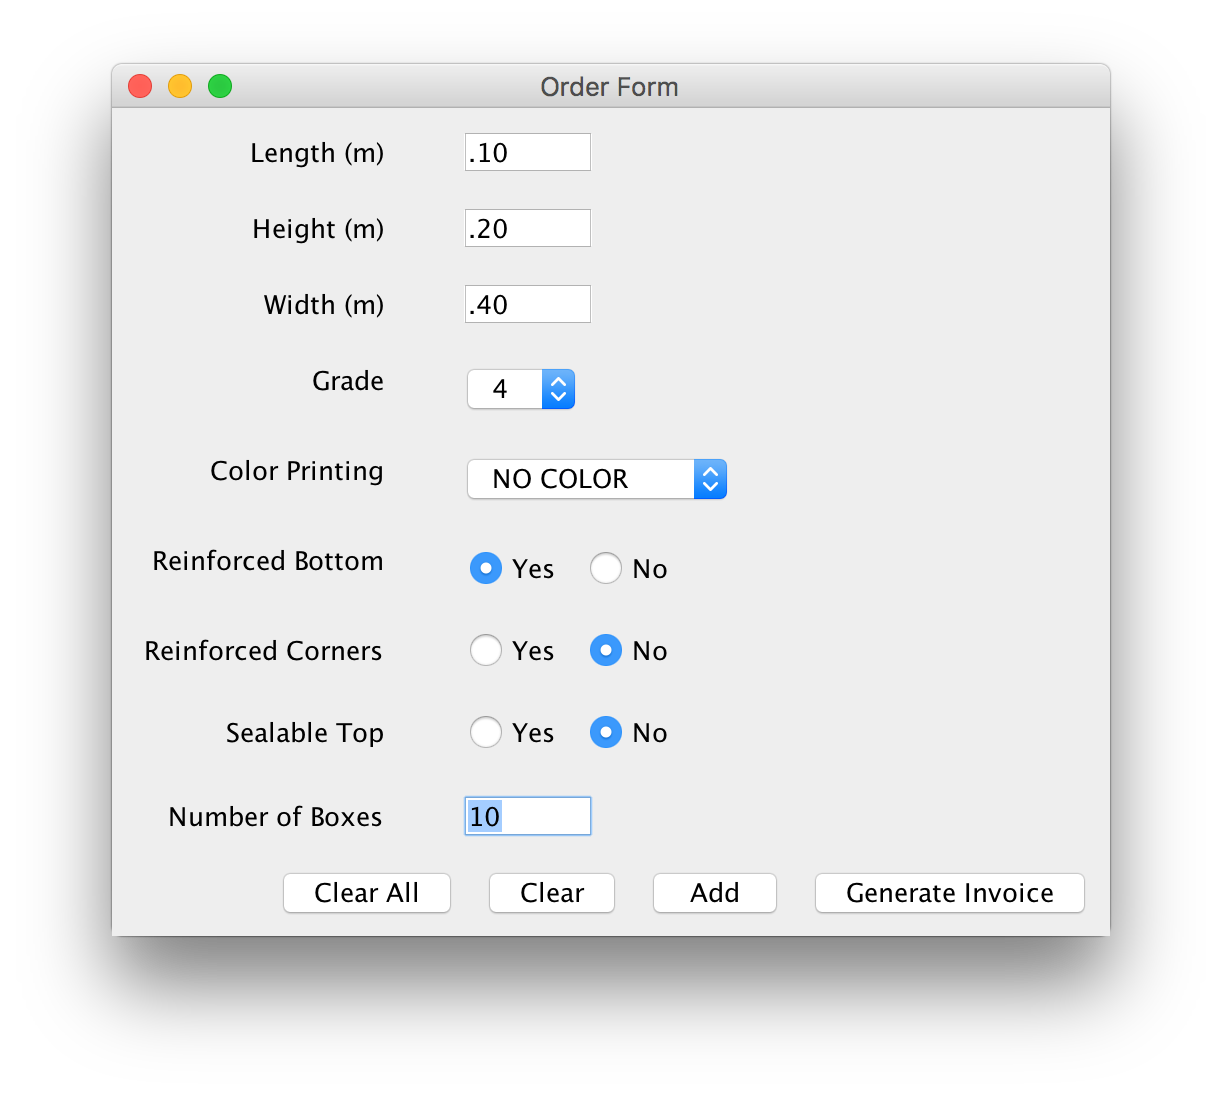
\includegraphics[width=\linewidth]{./screenshots/test_case_3_input.png}
	\caption{Test Case 3 Input}
	\label{test_case_3_input}
\end{figure}
\begin{figure}[H]
	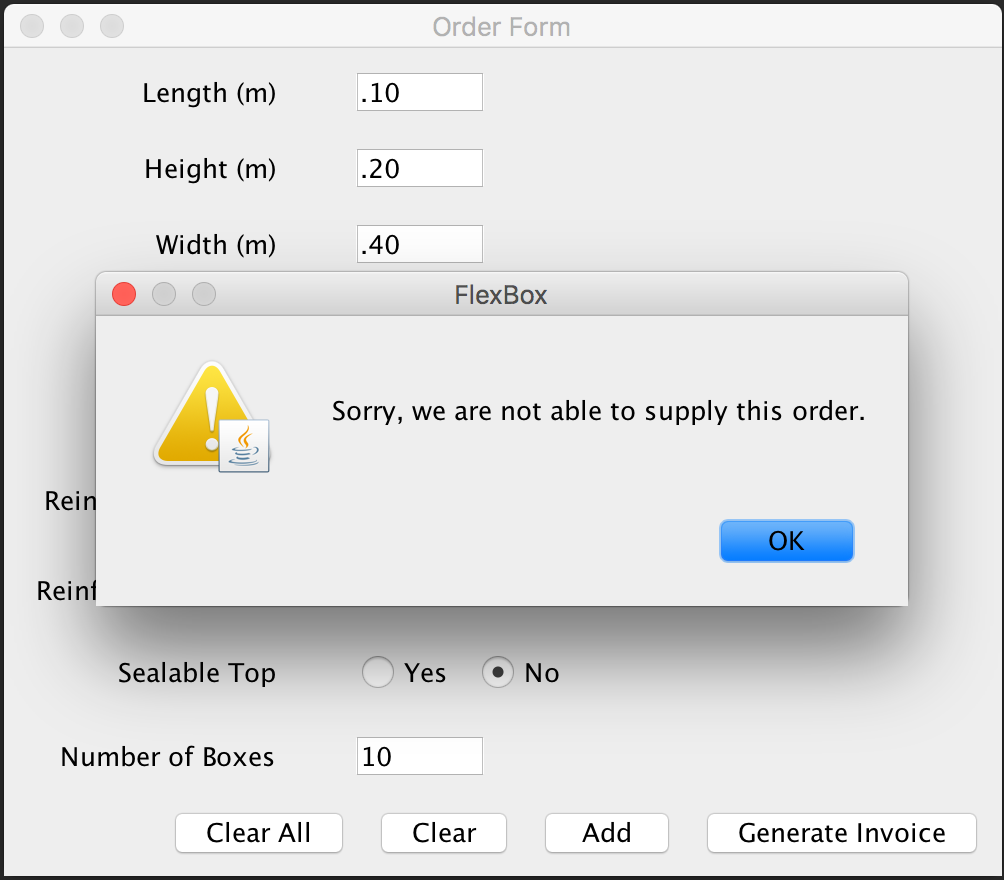
\includegraphics[width=\linewidth]{./screenshots/test_case_3_output.png}
	\caption{Test Case 3 Output}
	\label{test_case_3_output}
\end{figure}
\newpage
\subsection{Test 4}
\subsubsection{Test Case}
Generate invoice for empty order list
\subsubsection{Input}
Click 'Generate Invoice' button without adding any orders.
\subsubsection{Expected Output}
A popup showing error message "Please add your order before generating the invoice"
\subsubsection{Screenshots}
\begin{figure}[H]
	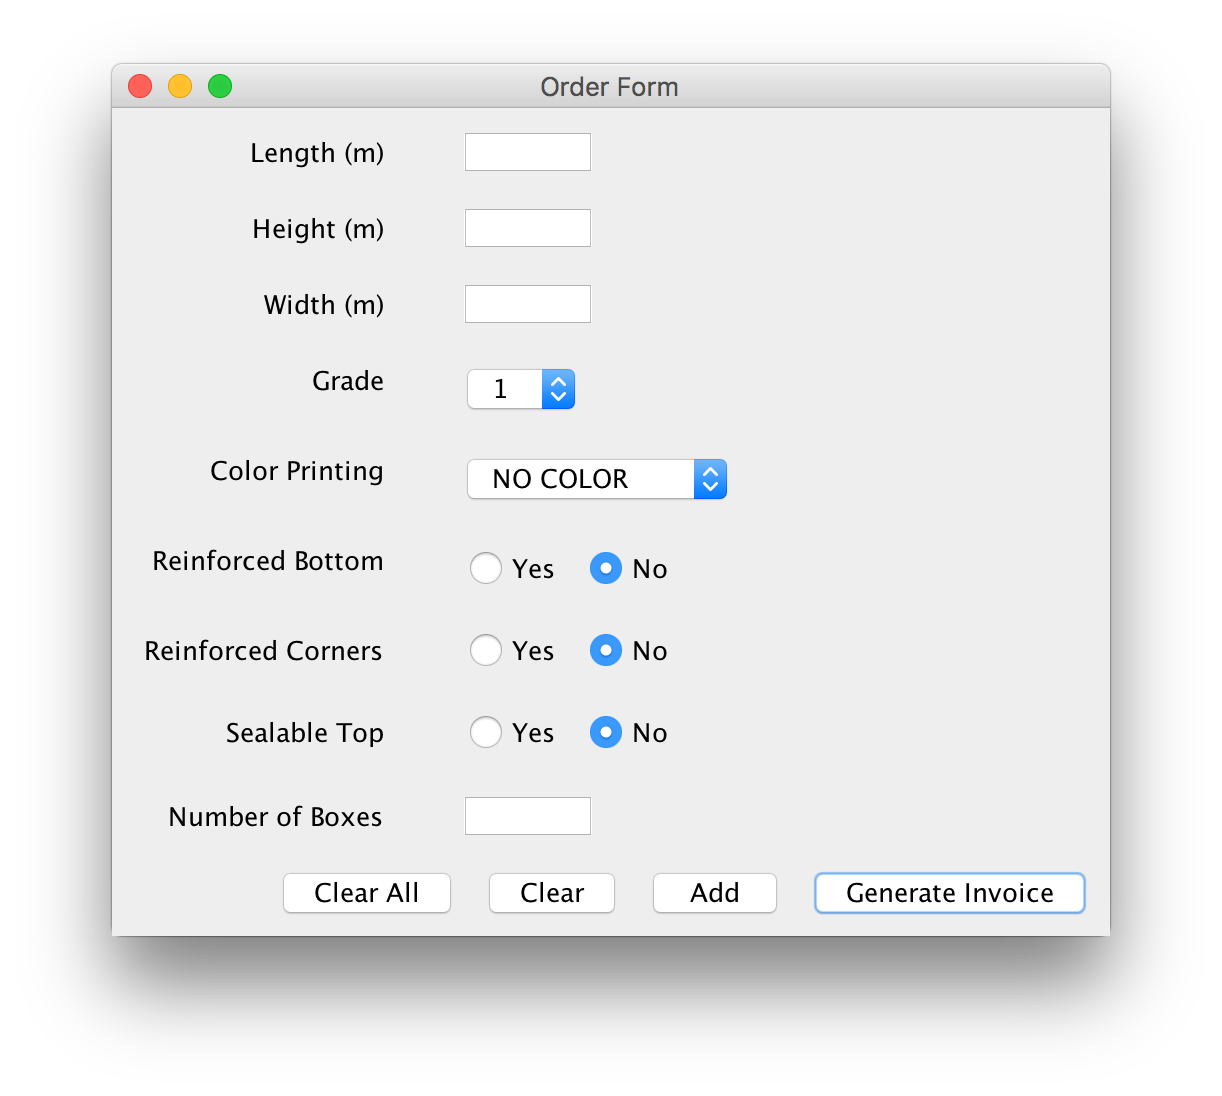
\includegraphics[width=\linewidth]{./screenshots/test_case_4_input.png}
	\caption{Test Case 4 Input}
	\label{test_case_4_input}
\end{figure}
\begin{figure}[H]
	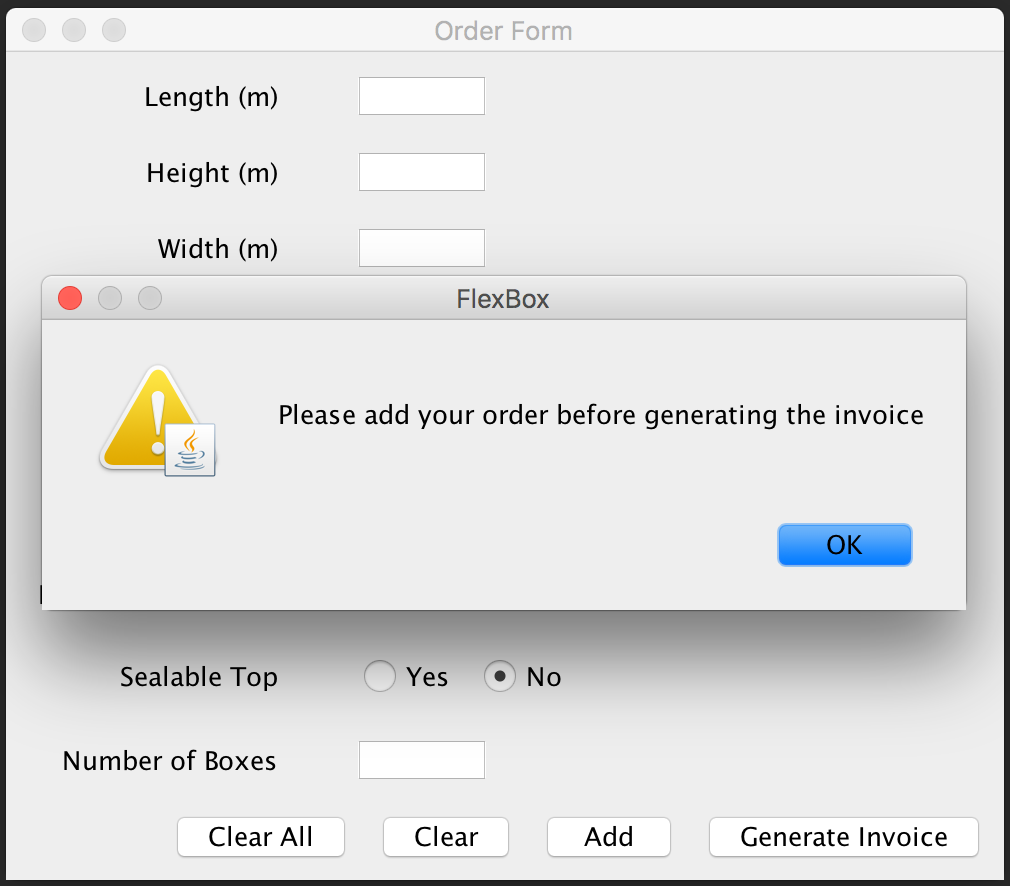
\includegraphics[width=\linewidth]{./screenshots/test_case_4_output.png}
	\caption{Test Case 4 Output}
	\label{test_case_4_output}
\end{figure}
\newpage
\subsection{Test 5}
\subsubsection{Test Case}
Single Order invoice
\subsubsection{Input}
Length: 0.20\\
Height: 0.30\\
Widht: 0.25\\
Grade: 3\\
Color Printing: TWO COLORS\\
Reinforced Bottom: Yes\\
Reinforced Corner: Yes\\
Sealable Top: No\\
Number of Boxes: 10\\
\subsubsection{Expected Output}
A popup showing info message "Order added successfully".
Invoice for the order.
\subsubsection{Screenshots}
\begin{figure}[H]
	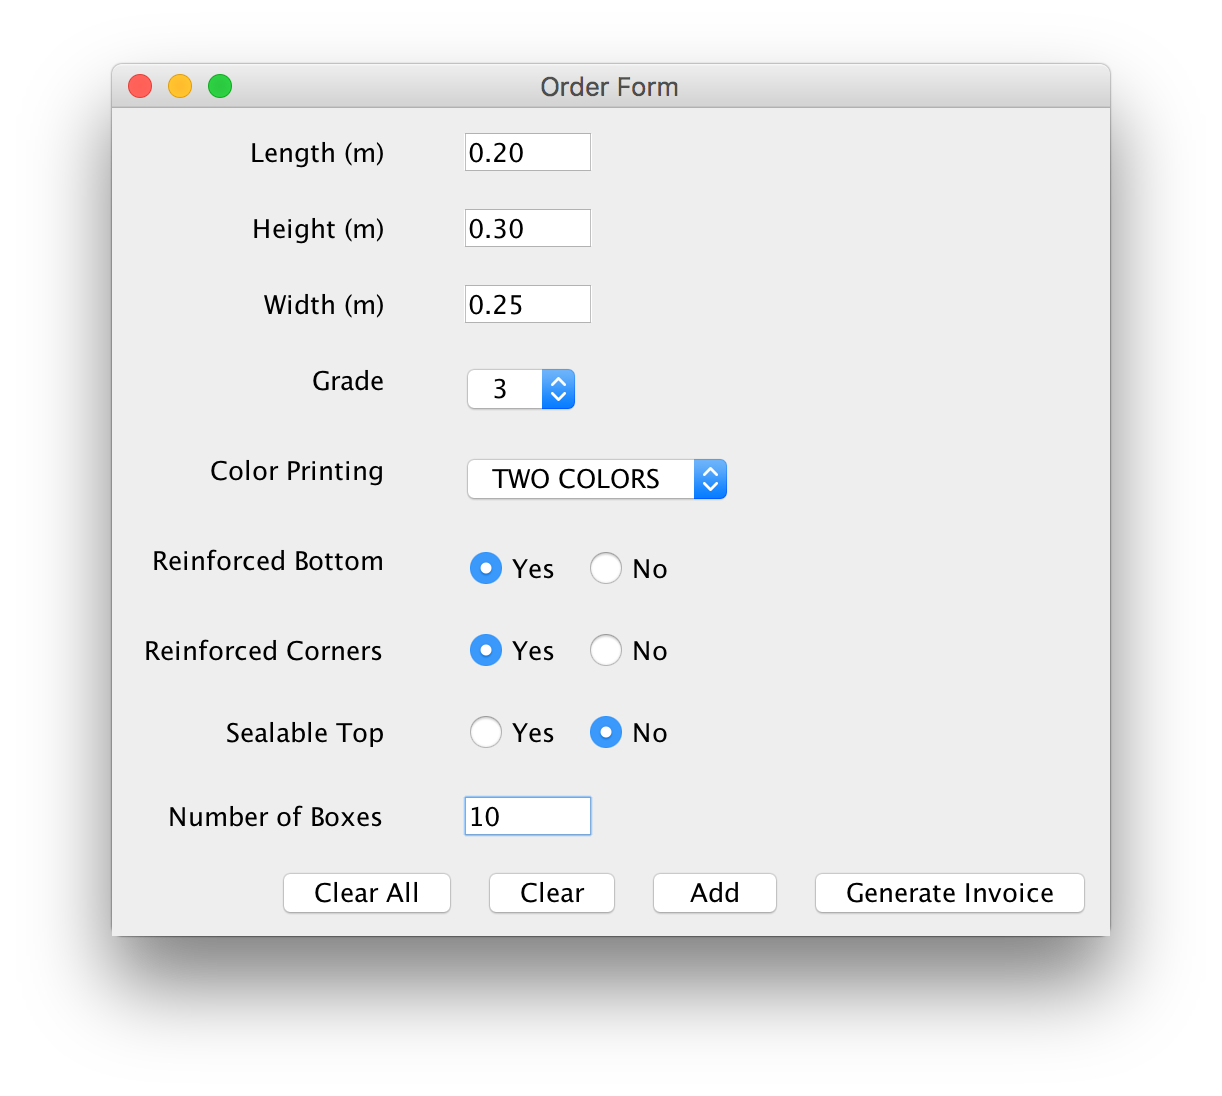
\includegraphics[width=\linewidth]{./screenshots/test_case_5_input.png}
	\caption{Test Case 5 Input}
	\label{test_case_5_input}
\end{figure}
\begin{figure}[H]
	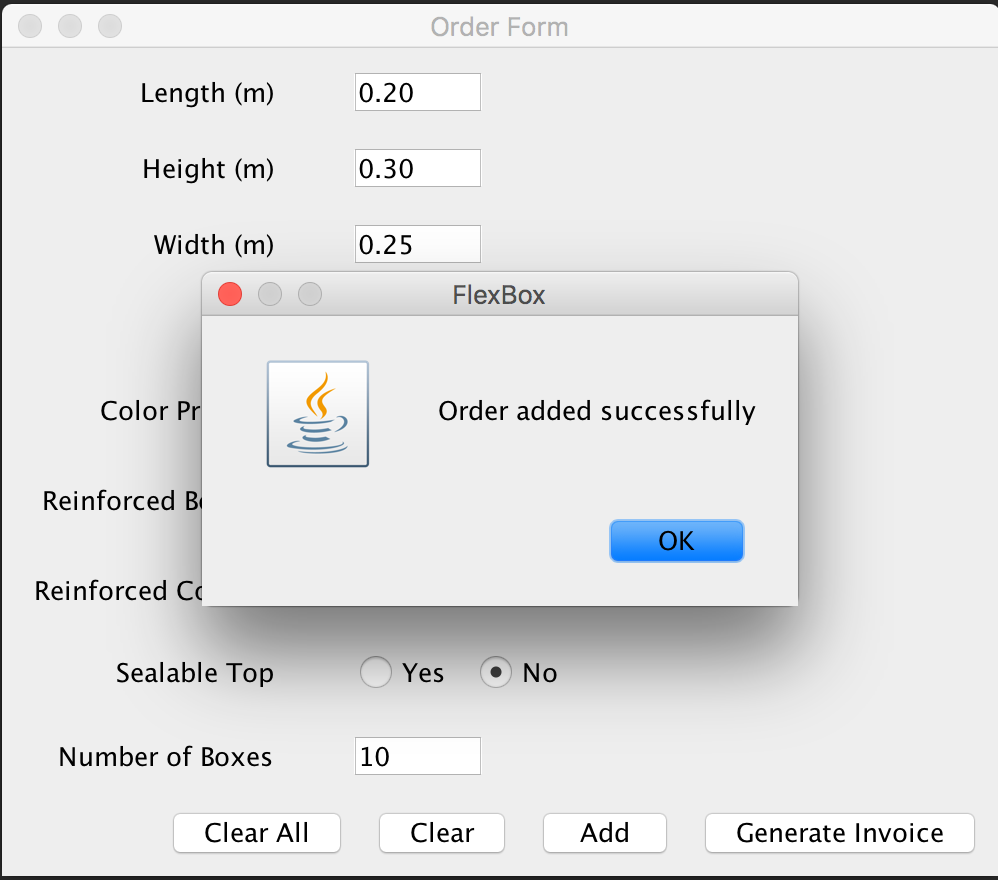
\includegraphics[width=\linewidth]{./screenshots/test_case_5_output_1.png}
	\caption{Test Case 5 Output 1}
	\label{test_case_5_output}
\end{figure}
\begin{figure}[H]
	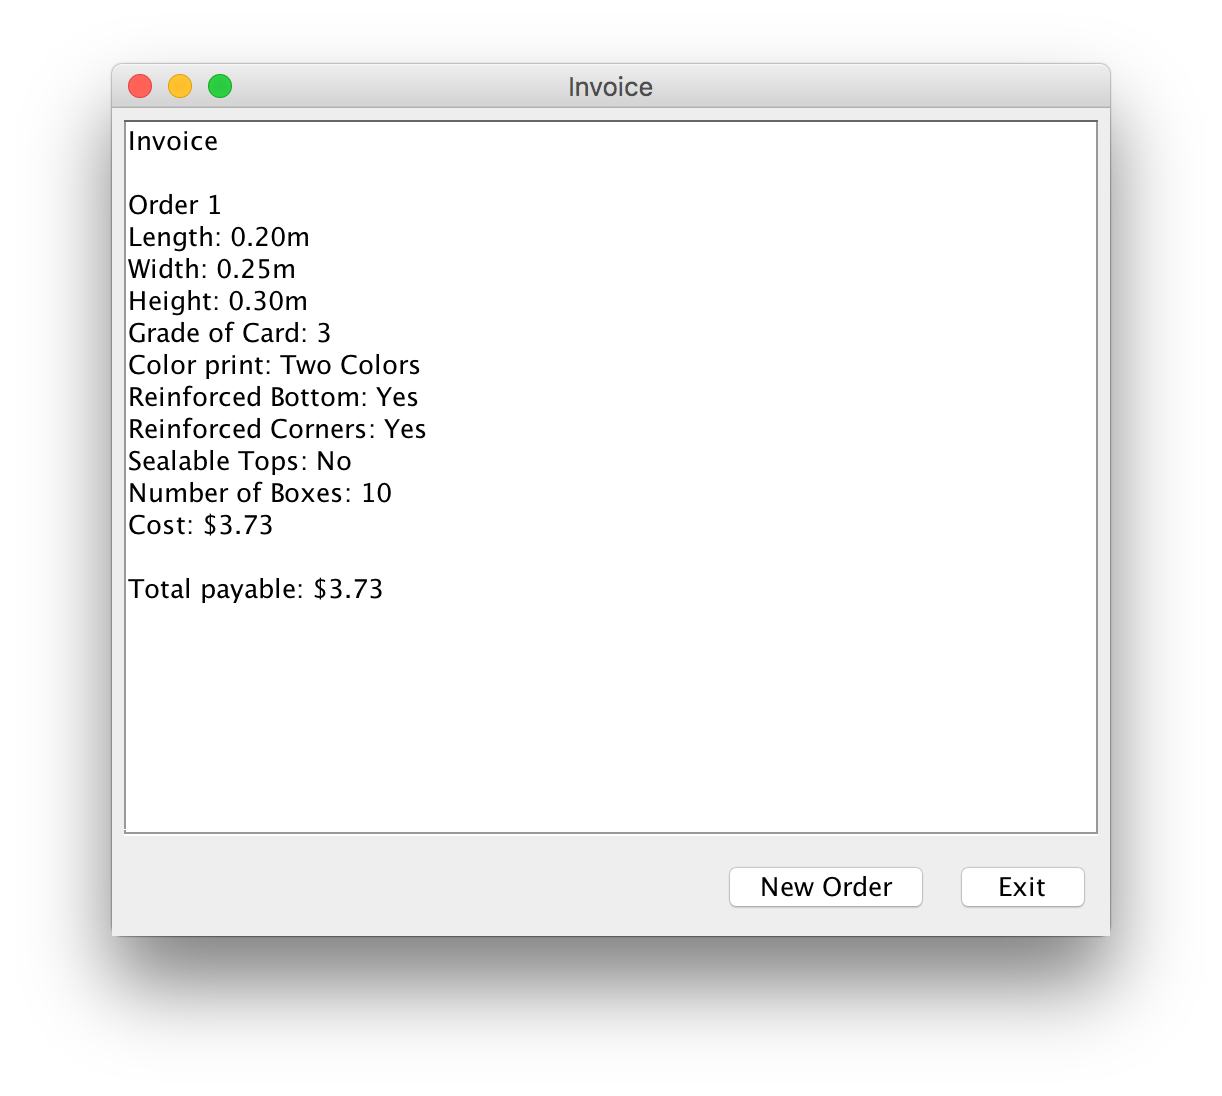
\includegraphics[width=\linewidth]{./screenshots/test_case_5_output_2.png}
	\caption{Test Case 5 Output 2}
	\label{test_case_5_output}
\end{figure}
\newpage
\subsection{Test 6}
\subsubsection{Test Case}
Multiple orders in same invoice
\subsubsection{Input}
\textbf{Order 1}\\
Length: 0.20\\
Height: 0.30\\
Widht: 0.25\\
Grade: 3\\
Color Printing: TWO COLORS\\
Reinforced Bottom: Yes\\
Reinforced Corner: No\\
Sealable Top: No\\
Number of Boxes: 15\\

Order 2\\
Length: 0.25\\
Height: 0.30\\
Widht: 0.15\\
Grade: 5\\
Color Printing: TWO COLORS\\
Reinforced Bottom: Yes\\
Reinforced Corner: Yes\\
Sealable Top: No\\
Number of Boxes: 10\\

Order 3\\
Length: 0.20\\
Height: 0.30\\
Widht: 0.25\\
Grade: 1\\
Color Printing: NO COLORS\\
Reinforced Bottom: No\\
Reinforced Corner: No\\
Sealable Top: Yes\\
Number of Boxes: 20\\
\subsubsection{Expected Output}
A "Order added successfully" popup for each oder.\\
Single invoice for all the three orders.
\subsubsection{Screenshots}
\begin{figure}[H]
	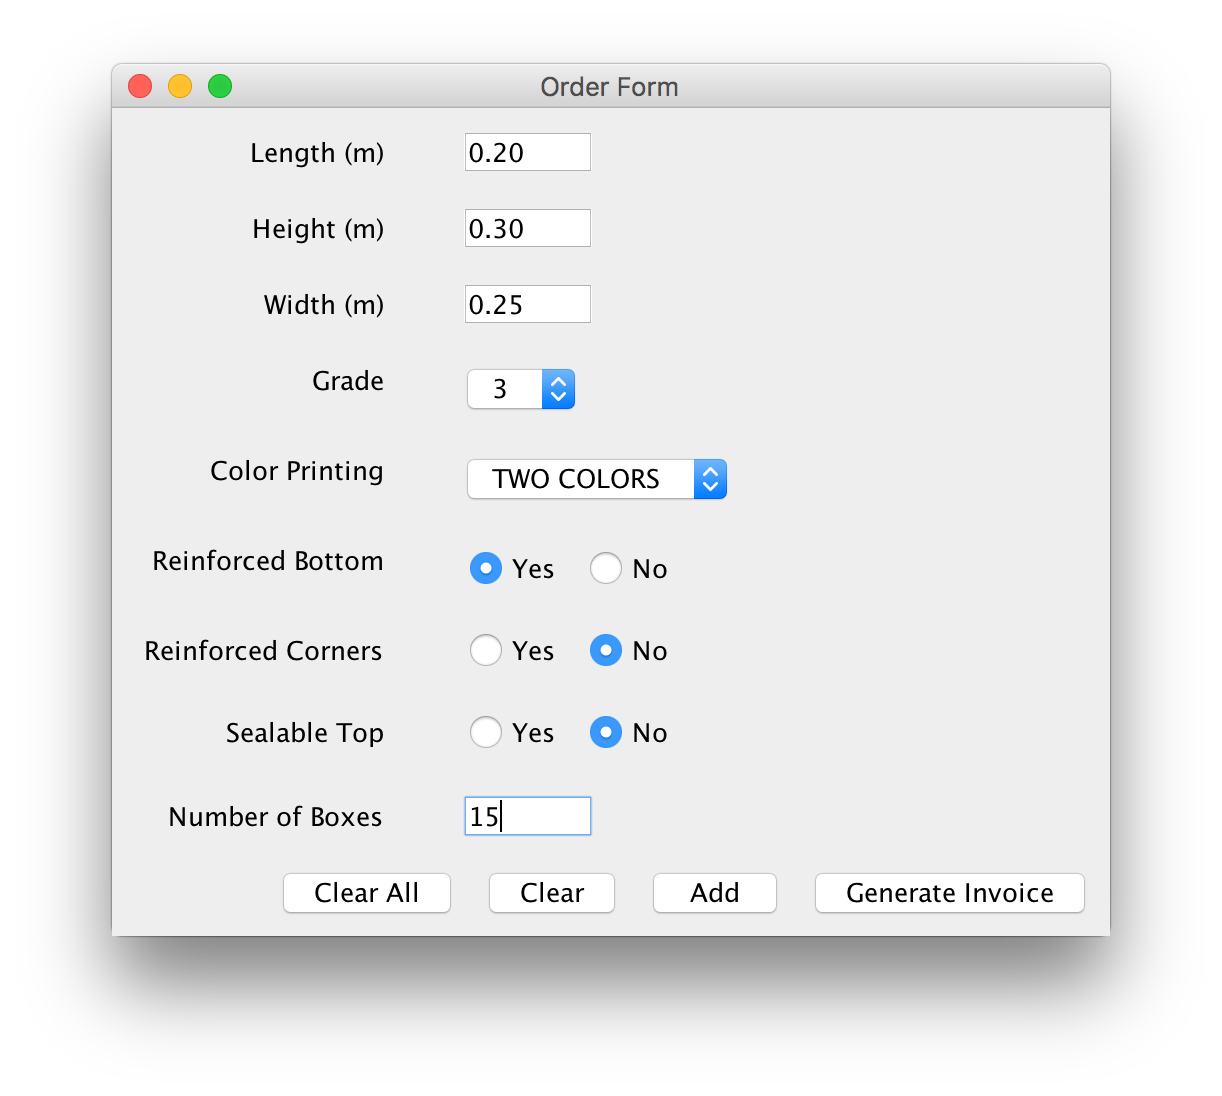
\includegraphics[width=\linewidth]{./screenshots/test_case_6_order1_input.png}
	\caption{Test Case 6 Input 1}
	\label{test_case_6_input_1}
\end{figure}
\begin{figure}[H]
	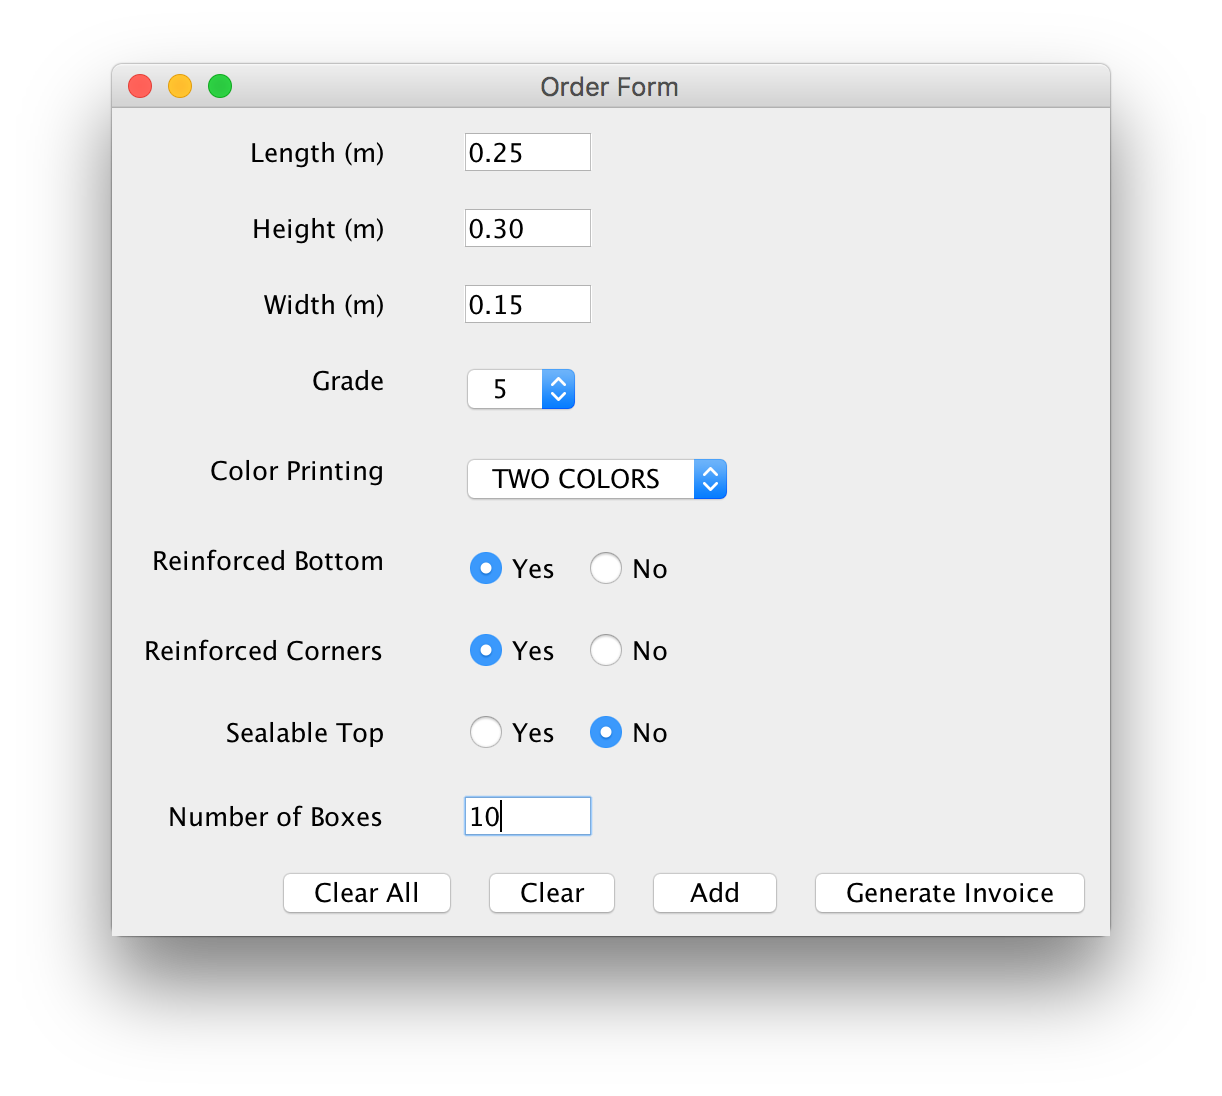
\includegraphics[width=\linewidth]{./screenshots/test_case_6_order2_input.png}
	\caption{Test Case 6 Input 2}
	\label{test_case_6_input_2}
\end{figure}
\begin{figure}[H]
	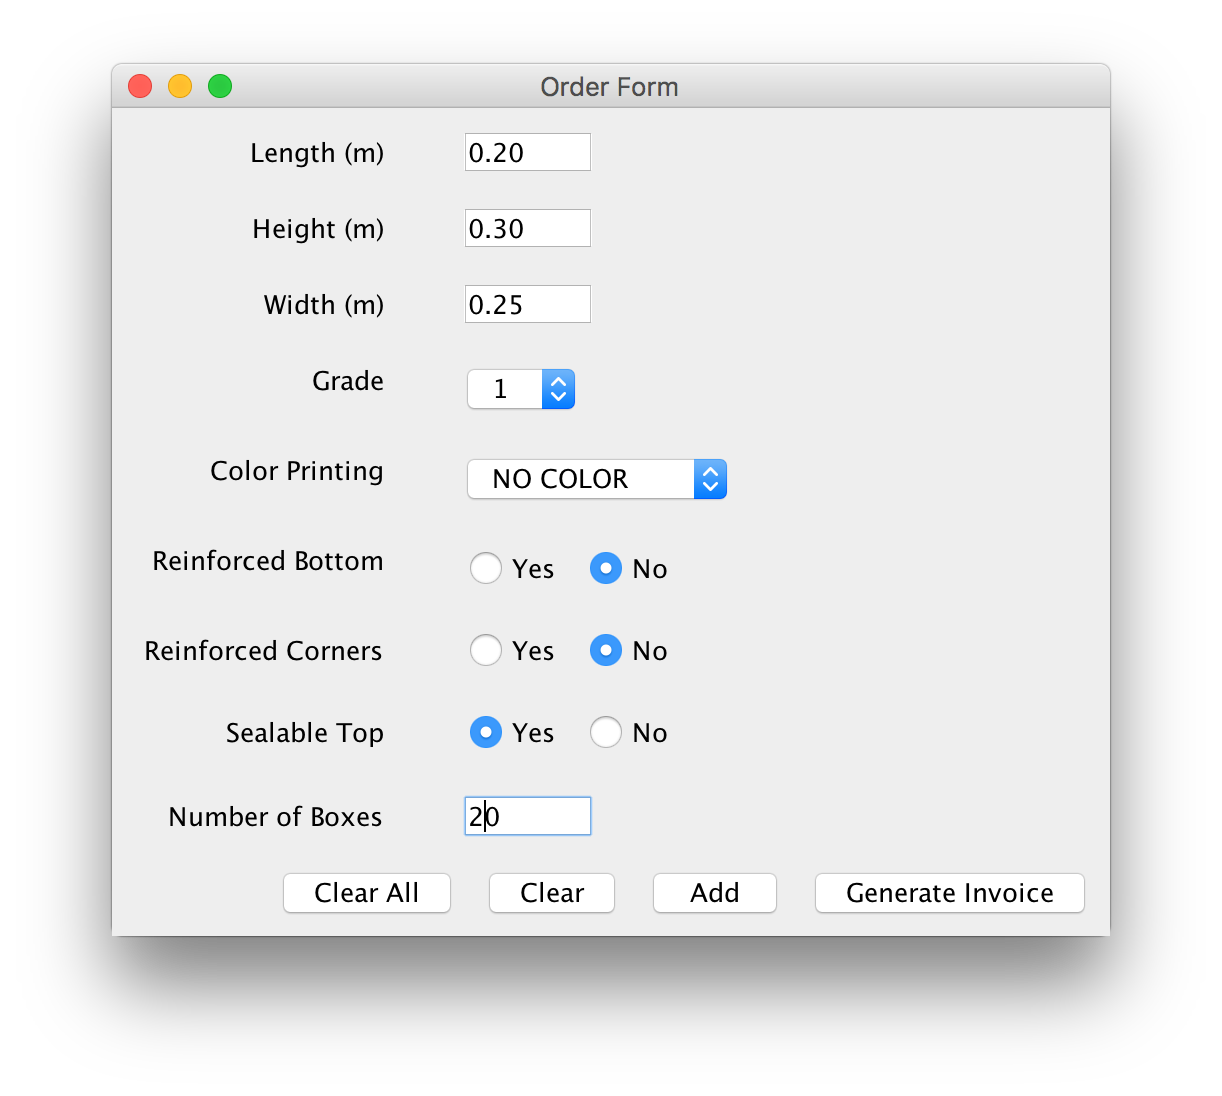
\includegraphics[width=\linewidth]{./screenshots/test_case_6_order3_input.png}
	\caption{Test Case 6 Input 3}
	\label{test_case_6_input_3}
\end{figure}
\begin{figure}[H]
	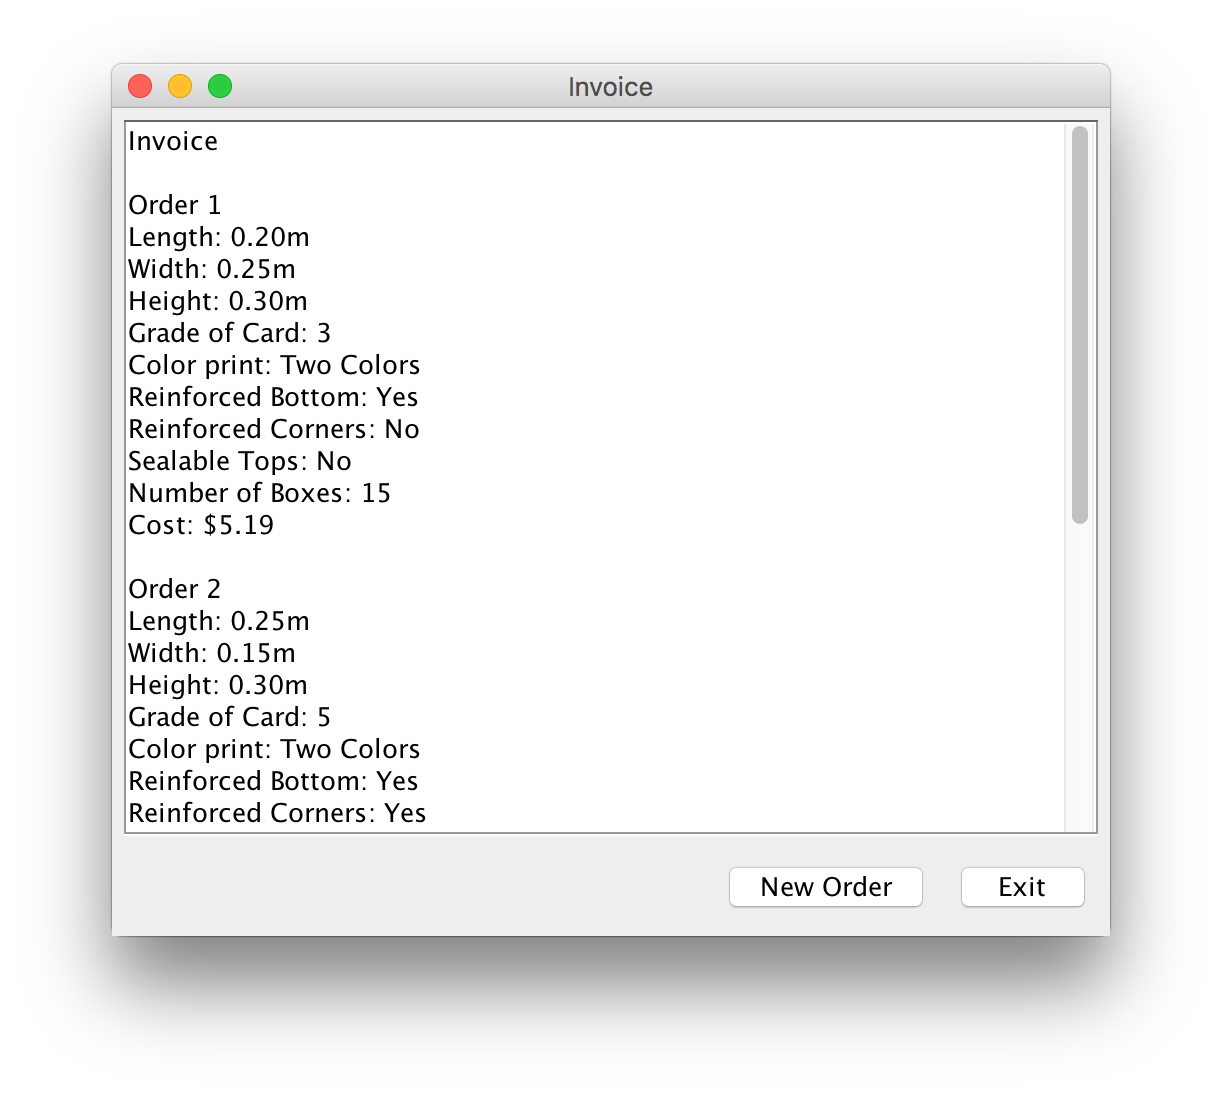
\includegraphics[width=\linewidth]{./screenshots/test_case_6_output_part1.png}
	\caption{Test Case 6 Output Part 1}
	\label{test_case_6_output}
\end{figure}
\begin{figure}[H]
	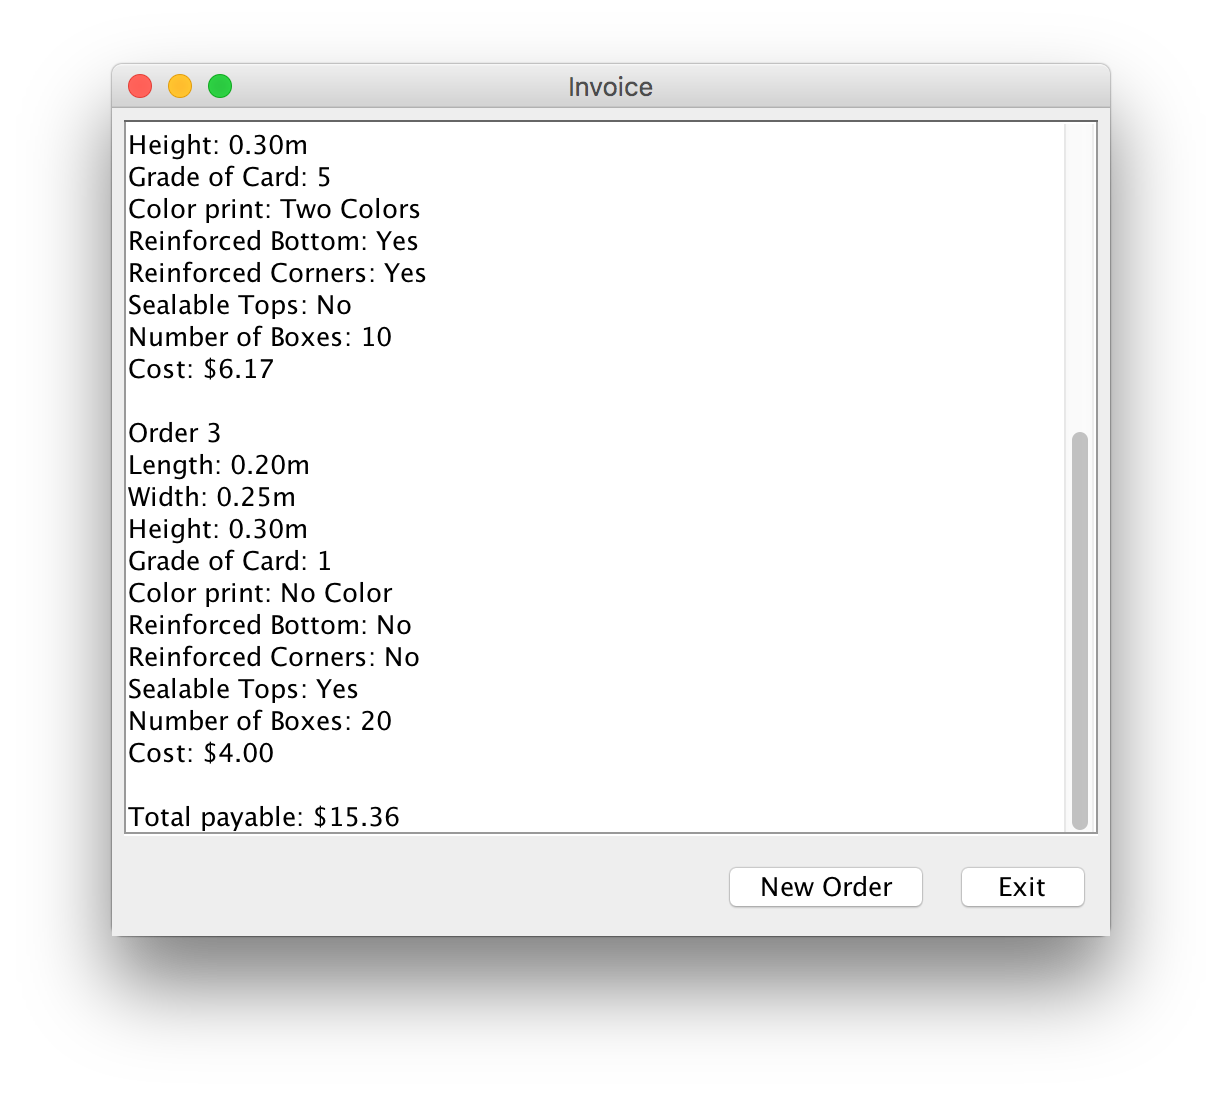
\includegraphics[width=\linewidth]{./screenshots/test_case_6_output_part2.png}
	\caption{Test Case 6 Output Part 2}
	\label{test_case_6_output}
\end{figure}
\newpage
\clearpage
\section{Sample Inputs and Outputs}
\subsection{Set 1}
\subsubsection{Input}
Length: 0.25\\
Height: 0.30\\
Width: 0.20\\
Grade: 2\\
Color Printing: ONE COLOR\\
Reinforcement Bottom: No\\
Reinforcement Corners: No\\
Sealable Top: Yes\\
Number of Boxes: 10\\
\subsubsection{Output}
Invoice\\
\\
Order 1\\
Length: 0.25m\\
Width: 0.20m\\
Height: 0.30m\\
Grade of Card: 2\\
Color print: No Color\\
Reinforced Bottom: No\\
Reinforced Corners: No\\
Sealable Tops: Yes\\
Number of Boxes: 10\\
Cost: \$2.40\\
\\
Total payable: \$2.40\\
\subsection{Set 2}
\subsubsection{Input}
Length: 0.20\\
Height: 0.30\\
Width: 0.40\\
Grade: 4\\
Color Printing: TWO COLORS\\
Reinforcement Bottom: Yes\\
Reinforcement Corners: No\\
Sealable Top: No\\
Number of Boxes: 15\\
\subsubsection{Output}
Invoice\\
\\
Order 1\\
Length: 0.20m\\
Width: 0.40m\\
Height: 0.30m\\
Grade of Card: 4\\
Color print: Two Colors\\
Reinforced Bottom: Yes\\
Reinforced Corners: No\\
Sealable Tops: No\\
Number of Boxes: 15\\
Cost: \$9.13\\
\\
Total payable: \$9.13\\
\subsection{Set 2}
\subsubsection{Input}
Length: 0.15\\
Height: 0.20\\
Width: 0.10\\
Grade: 1\\
Color Printing: ONE COLOR\\
Reinforcement Bottom: No\\
Reinforcement Corners: No\\
Sealable Top: Yes\\
Number of Boxes: 15\\
\\
Length: 0.25\\
Height: 0.25\\
Width: 0.40\\
Grade: 4\\
Color Printing: TWO COLORS\\
Reinforcement Bottom: Yes\\
Reinforcement Corners: Yes\\
Sealable Top: No\\
Number of Boxes: 25\\
\subsubsection{Output}
Invoice\\
\\
Order 1\\
Length: 0.15m\\
Width: 0.10m\\
Height: 0.20m\\
Grade of Card: 1\\
Color print: No Color\\
Reinforced Bottom: No\\
Reinforced Corners: No\\
Sealable Tops: Yes\\
Number of Boxes: 15\\
Cost: \$1.05\\
\\
Order 2\\
Length: 0.25m\\
Width: 0.40m\\
Height: 0.25m\\
Grade of Card: 4\\
Color print: Two Colors\\
Reinforced Bottom: Yes\\
Reinforced Corners: Yes\\
Sealable Tops: No\\
Number of Boxes: 25\\
Cost: \$16.54\\
\\
Total payable: \$17.59\\
\section{Appendix}
\subsection{FlexBox.java}
\lstinputlisting{./FlexBox/src/flexbox/FlexBox.java}
\newpage
\subsection{InvalidInputException.java}
\lstinputlisting{./FlexBox/src/flexbox/InvalidInputException.java}
\newpage
\subsection{View.java}
\lstinputlisting{./FlexBox/src/flexbox/View.java}
\newpage
\subsection{OrderFormWindow.java}
\lstinputlisting{./FlexBox/src/flexbox/OrderFormWindow.java}
\newpage
\subsection{InvoiceWindow.java}
\lstinputlisting{./FlexBox/src/flexbox/InvoiceWindow.java}
\newpage
\subsection{Model.java}
\lstinputlisting{./FlexBox/src/flexbox/Model.java}
\newpage
\subsection{OrderDetails.java}
\lstinputlisting{./FlexBox/src/flexbox/OrderDetails.java}
\newpage
\subsection{BoxTypeOne.java}
\lstinputlisting{./FlexBox/src/flexbox/BoxTypeOne.java}
\newpage
\subsection{BoxTypeTwo.java}
\lstinputlisting{./FlexBox/src/flexbox/BoxTypeTwo.java}
\newpage
\subsection{BoxTypeThree.java}
\lstinputlisting{./FlexBox/src/flexbox/BoxTypeThree.java}
\newpage
\subsection{BoxTypeFour.java}
\lstinputlisting{./FlexBox/src/flexbox/BoxTypeFour.java}
\newpage
\subsection{BoxTypeFive.java}
\lstinputlisting{./FlexBox/src/flexbox/BoxTypeFive.java}
\newpage
\subsection{Controller.java}
\lstinputlisting{./FlexBox/src/flexbox/Controller.java}
\end{document}